\documentclass{beamer}


% Load essential packages
\usepackage{hyperref} % Only load once to avoid conflicts
\usepackage{stile}
\usepackage{subcaption}
\usepackage{tcolorbox}
\usepackage[font=scriptsize,skip=1pt]{caption}
\usepackage[T1]{fontenc}
\usepackage{csquotes}
\usepackage[backend=biber, style=authoryear, maxnames=3, minnames=1, abbreviate=false, date=long, url=false, isbn=false, doi=false]{biblatex}
\addbibresource{lecture1/bib.bib} % Ensure this matches your bibliography file name

\interfootnotelinepenalty=10000

\usepackage{latexsym, amsmath, xcolor, multicol, booktabs, calligra}
\usepackage{graphicx, pstricks, listings, stackengine}

% Hyperref setup
\hypersetup{
    hidelinks,
    colorlinks=true,
    linkcolor=black,
    citecolor=deepblue,
    urlcolor=black
}

% Font theme for Beamer
\usefonttheme[onlymath]{serif}

% Custom definitions
\def\cmd#1{\texttt{\color{red}\footnotesize $\backslash$#1}}
\def\env#1{\texttt{\color{blue}\footnotesize #1}}
\definecolor{deepblue}{rgb}{0,0,0.5}
\definecolor{deepred}{rgb}{0.6,0,0}
\definecolor{deepgreen}{rgb}{0,0.5,0}
\definecolor{halfgray}{gray}{0.55}

% Beamer color settings
\setbeamercolor{block title}{bg=blue!70!white, fg=white}
\setbeamercolor{block body}{bg=blue!10!halfgray, fg=white}
\setbeamercolor{section in head/foot}{fg=white}
\setbeamercolor{subsection in head/foot}{fg=white}
\setbeamercolor{title in head/foot}{fg=white}


% Listings settings for code highlighting
\lstset{
    basicstyle=\ttfamily\small,
    keywordstyle=\bfseries\color{deepblue},
    emphstyle=\ttfamily\color{deepred},
    stringstyle=\color{deepgreen},
    numbers=left,
    numberstyle=\small\color{halfgray},
    rulesepcolor=\color{red!20!green!20!blue!20},
    frame=shadowbox,
}

\author{Freya Rubel}
\title{Trade, Migration and Global Challenges}
\subtitle{Introduction to Globalization - Questions}
\institute{}
\date{27.10.2026}

\graphicspath{{lecture1/}}

\begin{document}

\begin{frame}
    \titlepage
\end{frame}

\begin{frame}
    \tableofcontents[sectionstyle=show, subsectionstyle=show/shaded/hide, subsubsectionstyle=show/shaded/hide]
\end{frame}

\section{Technology and Accelerated Globalization}

\begin{frame}{Question 1}
    \textit{How does or did technology accelerate globalization?} \pause 
\begin{enumerate}
    \item \textbf{Lower transportation cost}: containerization, larger ships, and jet aircraft reduce per-unit shipping costs
    \item \textbf{Lower communication and coordination costs}: telecommunications and the internet make it cheaper to coordinate geographically distant producers and consumers, as well as production processes
    \item \textbf{Tradability of services and digital goods}: software, consulting, media, etc. can be distributed no matter the geographical distance
\end{enumerate}
\end{frame}

\section{KOF Globalization Index and Brexit}
\begin{frame}{Question 2}
 \textit{Does the KOF Global index of the UK change after Brexit?} \pause 
 \begin{figure}
     \centering
     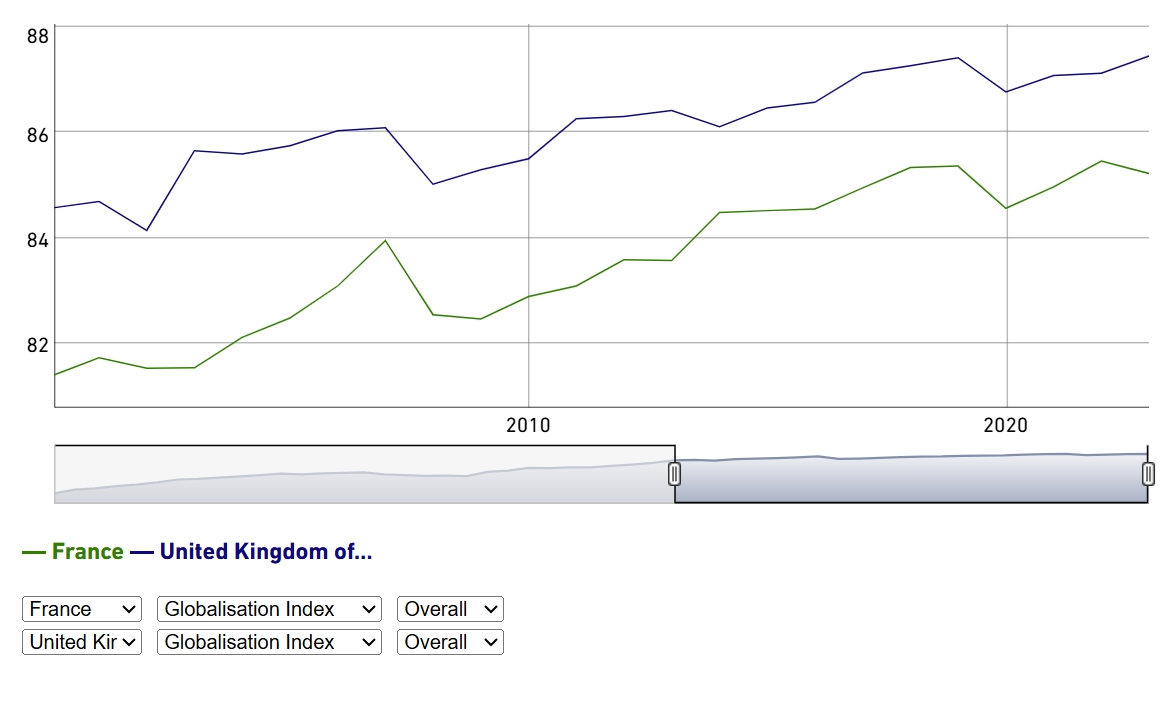
\includegraphics[width=0.9\linewidth]{lecture1/KOF_Brexit.png}
     \label{fig:placeholder}
 \end{figure}    
\end{frame}

\begin{frame}{Question 2}
    \begin{itemize}
        \item Economic Dimension:
        \begin{itemize}
            \item Drop for all countries in 2020 (Covid-19)
             \item Increase until 2022, afterwards decrease
        \end{itemize}
        \item Social Dimension:
        \begin{itemize}
            \item No detectable effect
            \item Long-term trend: slight upwards 
        \end{itemize}
        \item Political Dimension:
        \begin{itemize}
            \item Drop in the UK, no drop in other comparable countries
        \end{itemize}
    \end{itemize}
\end{frame}


 
 
\end{document}